%! Mode:: "TeX:UTF-8"
%! TEX program = xelatex
\PassOptionsToPackage{quiet}{xeCJK}
\documentclass[withoutpreface,bwprint]{cumcmthesis}
\usepackage{etoolbox}
\BeforeBeginEnvironment{tabular}{\zihao{-5}}
\usepackage[numbers,sort&compress]{natbib}  % 文献管理宏包
\usepackage[framemethod=TikZ]{mdframed}  % 框架宏包
\usepackage{url}  % 网页链接宏包
\usepackage{subcaption}  % 子图宏包
\usepackage{graphicx}
\usepackage{booktabs,colortbl}
\usepackage{xcolor}
\usepackage{xcolor}
\usepackage{tikz}
\usepackage{array}
\newcommand{\headcol}[1]{\textbf{#1}} % 假设你想要加粗表格的表头列
\tikzstyle{point}=[coordinate,on grid,]  
\usetikzlibrary{arrows,shapes,chains}
\usetikzlibrary{positioning, shapes.geometric,arrows,chains}
\usetikzlibrary{shapes.geometric, arrows,chains} 
\usepackage{indentfirst}
\usepackage{amsmath}
\newcolumntype{C}{>{\centering\arraybackslash}X}
\newcolumntype{R}{>{\raggedleft\arraybackslash}X}
\newcolumntype{L}{>{\raggedright\arraybackslash}X}
\usepackage{tikz}
\usepackage{listings}
\usepackage{xcolor} % 可选,用于代码高亮
\usetikzlibrary{arrows.meta} % 加载箭头元库


\title{基于数值分析的“板凳龙”路径仿真\\}  % 论文标题
\tihao{}  % 题号
\baominghao{}  % 报名号
\schoolname{}  % 学校
\membera{}  % 队员a
\memberb{}  % 队员b
\memberc{}  % 队员c
\supervisor{}  % 指导老师
\yearinput{}
\monthinput{}
\dayinput{}
%\small{顾晨曦 Chenxi.Gu22@student.xjtlu.edu.cn}\\\small{范訸然 Heran.Fan22@student.xjtlu.edu.cn}\\\small{须一菲 Yifei.Xu2202@}student.xjtlu.edu.cn\\
%%%%%%%%%%%%%%%%%%%%%%%%%%%%%%%%%%%%%%%%%%%%%%%%%%%%%%%%%%%%%
%% 正文
\begin{document}
\maketitle
\begin{abstract}
	本模型核心在于通过数学建模方法对传统民俗活动——板凳龙进行仿真模拟,为板凳龙中“盘龙”线路规划提出合理建议以优化其表演路径,提高安全性和观赏性。
	
	\textbf{对于问题一,}首先,明确螺线的具体类型,确立参数方程的研究方向;其次,由内至外求出给定圈数和总弧长;之后,通过对牛顿迭代和微元法思想的运用,用数值方法求解龙头前把手每个时刻的位置与速度。通过分析相邻节点之间的速度和位置关系,本研究建立了递推模型,描述并求解板凳龙在盘入螺旋路径过程中的动态变化。
	
	\textbf{对于问题二,}我们系统的考虑可能发生的碰撞情况,在二维空间中考虑直径卡滞和板板碰撞的情况并同时在三维空间中探索当板凳间有高度差时是否有把手碰撞板面可能性。将其转换为可量化的不等式条件,通过第一问获取的具体信息分别进行求解,并对结果进行对比分析,获取使得板凳之间不发生碰撞的最大终止时刻。
	
	\textbf{对于问题三,}根据题中最小化螺距需求确定优化目标函数,此优化模型的约束条件包括限定的掉头空间以及在第二个问题中通过计算得到的不发生碰撞的条件。据此建立用离散点逼近全局最优解的模型,通过在参数空间内系统地搜索离散点,逐步逼近全局最优解,得到满足条件的最小化螺距值。
	
	\textbf{对于问题四,}我们对于舞龙队盘入和盘出的过程,寻找使掉头路线最短的可能路径。在此基础上确定临界值,对整体时间范围进行分段拆分和模拟,通过运动学分析得到不同过程中前后板凳间的递推公式,求解每秒舞龙队的位置和速度。
	
	\textbf{对于问题五,}在前四问基础上进行总体分并在分段情况边界进行建模,求解出各时刻对应龙尾把手的位置,通过逆向工程方法逆推最小龙头速度,基于各把手的速度均不超过$2m/s$的条件下寻求最优速度配置方案。

	

	
	
%	本模型核心在于对黄灯相位周期内车辆行进过程的分段研究,并对合理黄灯时长的影响因子的作用进行具体探究,针对现行黄灯时长提出合理建议,针对问题一,我们采用控制变量方式,基于理想条件和现实参数分别建立匀速前进的模型一和变速的模型二,并对不同初速度机动车辆的不同情况进行分类。针对问题二,我们带入基于现实情况的各项参数数值,对计算得出的具体黄灯时长进行分析与现行较为普遍的$3-4s$进行对比分析。
%	
%\textbf{对于问题一,}首先,我们构建了基于理想化交通环境的黄灯时长数学模型;其次,我们考虑了实际交通条件下的参数变化,如驾驶员反应时间、不同车型和道路条件,进一步建立了模型二;同时对不同初速度机动车辆的不同情况进行分类,分别探究初速度和绿灯变黄灯时距停止线距离对合理黄灯时长的具体影响。
%
%\textbf{对于问题二,}利用控制变量法,分别探究有无黄灯倒计时,初速度大小,离停止线距离大小,行驶方向对于合理黄灯时长的影响,结果表明,在有黄灯倒计时,初速度更大,离停止线更远,直行情况下,为保证所有车辆都顺利通过交叉路口,应设置更久的黄灯时长来确保安全性。
%
%\textbf{对于问题三,}为评估模型下机动车通过交叉路口的效率,本研究计算了车辆通过本侧停止线与对侧停止线所需时间的相关系数。通过两两间相关系数的计算,我们能够量化车辆通过交叉口的相互依赖性。在此基础上进一步绘制了热力图以直观展示不同车辆间的时间关联性,验证模型的可行性和优越性,并进一步分析模型潜在优势,提出改进方向。
%
%结果表明,通过合理调整黄灯时长,可以显著提高车辆的通过率,减少交叉口内的交通事故。此外,我们还探讨了延长黄灯时长可能带来的潜在问题,如通行时间的不确定性增加和对交通流量的影响。
%本研究针对城市交通信号灯黄灯时长设置问题,采用数学建模和数据分析方法,对影响黄灯时长的关键因素进行了深入探讨。文章首先概述了黄灯在交通信号控制中的重要性及其在交通事故预防中的作用。通过对现有法规和驾驶员行为的分析,我们建立了考虑不同初始速度、行驶距离和反应时间等因素的数学模型,旨在优化黄灯时长设置,提高交叉口的通行效率和安全性。
%
%研究分为三个主要部分:首先,我们构建了基于理想化交通环境的黄灯时长数学模型;其次,我们考虑了实际交通条件下的参数变化,如驾驶员反应时间、不同车型和道路条件,进一步细化了模型;最后,我们将模型结果与现行标准进行比较,分析了模型的优势和局限性,并提出了优化建议。
%
%本研究的创新点在于综合考虑了多种影响因素,并通过实际数据验证了模型的有效性。结果表明,通过合理调整黄灯时长,可以显著提高车辆的通过率,减少交叉口内的交通事故。此外,我们还探讨了延长黄灯时长可能带来的潜在问题,如通行时间的不确定性增加和对交通流量的影响。

\keywords{仿真模拟\quad  线性规划  \quad 二分法 \quad 牛顿迭代 \quad 阿基米德螺线}
\end{abstract}
%%%%%%%%%%%%%%%%%%%%%%%%%%%%%%%%%%%%%%%%%%%%%%%%%%%%%%%%%%%%% 

\tableofcontents  % 目录
\newpage

%%%%%%%%%%%%%%%%%%%%%%%%%%%%%%%%%%%%%%%%%%%%%%%%%%%%%%%%%%%%%  
\section{问题重述}
\subsection{问题背景}
板凳龙是起源于浙闽地区的传统民俗活动之一,是当地人迎神、祈福的一项民俗活动,蕴含着深厚的地域文化。自改革开放以来,板凳龙迎来了传承与弘扬的新时期。现代板凳龙不仅保留了其传统特色,还逐渐发展成为一个综合性的艺术形式,巧妙地融合了书法、绘画、剪纸、刻花、雕塑等多种艺术手法,以及扎制、编糊等传统工艺,是重要的国家级非物质文化遗产。

盘龙作为板凳龙表演的一种特定形式,板凳龙队伍整体呈螺旋状排列。在此篇文章中,我们将以盘龙的表演形态为基础,对特定时间段内队伍中各个节点的位置、速度以及整体的螺距等关键指标进行探究。研究的目的是为了确定合理的螺距值,优化盘龙掉头时的行进路径。在确保表演安全性的基础上,提升板凳龙表演的娱乐性和观赏价值,从而增强其在文化推广和宣传方面的潜力。
%\begin{tikzpicture}[
%	% 定义粗箭头样式
%	thick_arrow/.style={
%		postaction={
%			-Stealth, % 使用Stealth箭头样式
%			draw,      % 绘制箭头
%			thick      % 设置箭头为粗线条
%		}
%	}
%	]
%	
%	% 画带粗箭头的直线
%
%\end{tikzpicture}
\subsection{问题要求}
\begin{itemize}
  \item \textcolor{black}{问题一: 固定盘龙的盘入轨迹为螺距为55$cm$的等距螺线,顺时针从第十六圈开始盘入,盘入过程中行进速度恒定为$1m/s$,需求出每秒板凳龙队伍所有节点的位置与速度,取$0-300s$中指定位置坐标与速度,将结果存入.xlsx文件并在文中给出要求关键值}
  \item \textcolor{black}{问题二:在确保队列沿预定螺线路径盘入且板凳之间不会发生碰撞情况下,确定合适的终止时刻(即临界点)队列中各节点的位置和速度。}
  \item \textcolor{black}{问题三:盘龙状态由盘入转变成逆时针掉头盘出状态,给定直径为 $r = 4.5m$ 的圆作为掉头区域,求解使龙头前把手能够沿着相应的螺线盘入到调头空间的边界成立时的最小螺距。}
  \item \textcolor{black}{问题四:在问题三给定掉头空间基础上,求解当盘入螺线的螺距为1.7$m$,盘出与盘入螺线关于螺线中心呈中心对称,前一段圆弧的半径是后一段的 2 倍,且与盘入、盘出螺线均相切的掉头曲线,使掉头弧线弧长变短。在龙头前把手保持 1 m/s情况下,求出从−100$s$-100$s$每秒板凳龙各节点的位置和速度。}
  \item \textcolor{black}{问题五:板凳龙沿问题 4 设定的路径行进且龙头行进速度保持不变,需确定龙头的最大
  	行进速度,使得舞龙队各把手的速度均不超过 2 m/s。}
\end{itemize}

%%%%%%%%%%%%%%%%%%%%%%%%%%%%%%%%%%%%%%%%%%%%%%%%%%%%%%%%%%%%% 

\section{问题分析}
\subsection{问题一的分析}
问题一首先需明确螺线的具体类型,并确立相应的数学参数方程。在此基础上,由内圈至外圈求出给定圈数和螺距下螺线线总弧长。进一步地,根据给定的恒定龙头行进速度,可逆向推出龙头行进距离,并基于极坐标写出每秒龙头位置(直角坐标系原点)。通过对该系统的运动学特性进行分析,可以建立板凳前后位置和速度的递推关系模型。带入计算程序,获取所需数据并写入表格。

\subsection{问题二的分析}
在题一解答的基础上,通过观察板凳龙运行过程中各节点的位置和速度,判断碰撞可能发生的情况,基于此求出不同可能情况下对应时间。选取更小的$t$值,即选取最先可能发生碰撞的情况作为本题解答。

\subsection{问题三的分析}
优化模型下,以等距螺线中螺距尽量大作为目标函数,第二问不碰撞条件以及掉头区域半径为约束函数,在满足约束条件的情况下,使得目标函数尽量大。进行逐步寻优,先确认半径,逐步寻找其他决策变量的优解,使得目标函数达到全局最优解。
 
\subsection{问题四的分析}
需依据题目所提供的条件,分段构建的$-100-100s$模拟掉头路径。在此基础上,利用基本不等式确定一条弧长相比更短的最优路径。此外,还需对板凳龙在进入掉头路线后,即在题目规定的$0-100s$内固定点的位置和速度进行分段详细分析。通过这一分析优化路径选择,确保在给定时间区间内实现最佳动态表现。

\subsection{问题五的分析}
基于问题四,总体分析同一时刻板凳龙各节点的速度以及同一节点随时间变化的趋势,在边界建立模型,基于各把手的速度均不超过$2m/s$的条件寻求最优速度配置方案。

%\begin{figure}
%	\centering
%	\begin{tikzpicture} [>=latex, scale = 0.8]
%		% 画半圆,中心在(0,0),半径为2cm
%		\draw (-3,2) arc (270:360:1cm);
%		\draw (-2,-3) arc (0:90:1cm);
%		\draw (2,3) arc (180:270:1cm);
%		\draw (3,-2) arc (90:180:1cm);
%		% 可以添加一些辅助线或标记
%		\fill (0,0) circle (2pt); % 标记圆心
%		\draw (3,2) -- (7,2); 
%		\draw (3,-2) -- (7,-2); 
%		\draw (-3,2) -- (-7,2); 
%		\draw (-3,-2) -- (-7,-2); 
%		\draw (2,3) -- (2,7); 
%		\draw (2,-3) -- (2,-7); 
%		\draw (-2,-3) -- (-2,-7); 
%		\draw (-2,3) -- (-2,7); 
%		\draw (-1,0) -- (1,0); % x轴
%		\draw (0,-1) -- (0,1); % y轴
%		\draw (0,3) -- (0,7); 
%		\draw (0,-3) -- (0,-7); 
%		\draw (3,0) -- (7,0); 
%		\draw (-3,0) -- (-7,0); 
%		\draw[line width=1.5pt, ->] (1,-4) -- (1,-2.2);
%		\draw[line width=1.5pt] (1.5,-4) -- (1.5,-2.7);
%		\draw[line width=1.5pt, ->] (1.5,-2.7) -- (1.8,-2.2);
%		\draw[line width=1.5pt] (1,-2.2) -- (1,-2);
%	\end{tikzpicture}
%\caption{双向三车道十字路口示意图}
%\end{figure}


%%%%%%%%%%%%%%%%%%%%%%%%%%%%%%%%%%%%%%%%%%%%%%%%%%%%%%%%%%%%% 

\section{模型假设}
\subsection{基本假设}
\begin{itemize}
	\item 假设板凳龙每一小节在进入题目描述的特定区域前,沿着与题目提供的相等恒定螺距的螺旋轨迹进行等距螺线运动。
	\item 假设所有把手中心位置都在给定等距螺线上,相邻板凳有两个把手的中心点连接。
	\item 假设板凳材料不具备受挤压收缩的性质,板凳间距离保持恒定。
	\item 假设每节板凳的速度连续,板凳间运动具有平滑性,可利用递推求出每个节点(把手)速度。
\end{itemize}
\subsection{问题一附加假设}
\begin{itemize}
	\item 假设板凳穿孔的直径对运动不造成影响,把手中心点可代表把手的运动轨迹。
  \item 假设不存在碰撞情况,龙头前把手可以盘入至直角坐标系原点。
  \item 假设相邻的前后板凳不存在高度差且手握把手的“舞龙人”不存在身高差,所有板凳均在同一二维平面,所有运动不涉及竖直方向上的运动。
\end{itemize}
\subsection{问题四附加假设}
\begin{itemize}
	\item 假设掉头轨迹半径以及掉头轨迹模型可根据题意进行简化。
	\item 假设龙头板凳长度无限接近于其他板凳长度。
\end{itemize}

\section{符号说明}
\subsection{问题一符号说明}
%tab1
\begin{table}[htb!]
  \centering
  \small
  \begin{tabular}{p{60pt}<{\centering}|p{60pt}<{\centering}p{180pt}<{\raggedright}}
   \hline
   \rowcolor{gray!25} % 设置行颜色为25%的灰色
   \headcol \textbf{序号} & \textbf{符号} & \textbf{符号说明} \\
   \hline
    1 & $a$ & 起点到极坐标原点的距离(m) \\
    2 & $b$ & 螺旋线每增加单位角度$r$随之对应增加的数值(m)  \\
    3 & $p$ & 螺距(m)\\
    4 & $\gamma$ &把手距螺线原点的弧度(rad)\\
    5 & $\theta$ &   把手行进弧度(rad)\\
    6 & $Q$ & 螺线圈数 \\
    7 & $d$ & 龙头距外圈距离最近的板凳的平面距离(m) \\
    8 & $S$ & 螺线总弧长(m) \\

%    10 & $P=\dfrac{\lambda}{\mu}$& 谣言传播强度\\
	\hline
  \end{tabular}
%  \caption{问题一符号与说明}
  \label{symbol}
\end{table}
\begin{table}[htb!]
	\centering
	\small
	\begin{tabular}{p{60pt}<{\centering}|p{60pt}<{\centering}p{180pt}<{\raggedright}}
		\hline
		\rowcolor{gray!25} % 设置行颜色为25%的灰色
		\headcol \textbf{序号} & \textbf{符号} & \textbf{符号说明} \\
		\hline
		9 & $\gamma_i$ & 第$i$个节点在某固定时刻对应弧度(rad) \\
		10 & $h$ & 步长(m) \\
		11 & $L_0$ & 龙头有效板长(2.86m) \\
		12 & $L_c$ & 除龙头外其他板有效板长(1.65m) \\
		13 & $w$& 模板宽度(0.3m)\\
		14 & $D$& 把手孔径($5.5*10^{-2}$m)\\
		15 & $\gamma_{head}$ & 把手距螺线原点的弧度(rad) \\
		16 & $t'$ & 步长,即走入一节板凳的时间周期(m)  \\
		%    10 & $P=\dfrac{\lambda}{\mu}$& 谣言传播强度\\
		\hline
	\end{tabular}
	%  \caption{问题一符号与说明}
	\label{symbol1}
\end{table}
%\subsection{问题二补充符号说明}
%%tab1
%\begin{table}[htb!]
%	\centering
%	\small
%	\begin{tabular}{p{60pt}<{\centering}|p{60pt}<{\centering}p{180pt}<{\raggedright}}
%		\hline
%		\headcol 序号 & 符号 & 符号说明 \\
%		\hline
%		1 & $j(t)$ & 谣言判断者总学生比重 \\
%		2 & $w(t)$ & 真实信息传播者占总学生比重\\
%		3 & $a$ & 单位时间内谣言未知者转化为谣言判断者人数(人/$H$)\\
%		4 & $b$ &单位时间内谣言未知者转化为信谣传谣者人数(人/$H$) \\
%		5 & $c$ & 单位时间内谣言未知者转化为真实信息传播者人数(人/$H$) \\
%		6 & $d$& 单位时间内谣言未知者转化为谣言免疫者人数(人/$H$)\\
%		7 & $e$& 单位时间内谣言判断者转化为信谣传谣者人数(人/$H$)\\
%		8 & $f$ & 单位时间内谣言判断者转化为真实信息传播者人数(人/$H$)) \\
%		9 & $g$ & 单位时间内谣言判断者转化为谣言免疫者人数(人/$H$)  \\
%		10 & $l$ & 单位时间内信谣传谣者转化为谣言免疫者人数(人/$H$)  \\
%		\hline
%	\end{tabular}
%%	\caption{问题二符号与说明}
%	\label{symbol2}
%\end{table}



 \newpage
\section{模型的建立与问题的求解}
\subsection{问题一模型的建立}
依据题意给出的等距条件,建立起有关阿基米德螺线的参数方程,在极坐标系中,螺线的方程\cite{ref1}为:
	$$r = a + b\gamma$$
	
其中,$a$为起点到极坐标原点的距离,$b$为螺旋线每增加单位角度$r$随之对应增加的数值,即$b = \frac{55}{2\pi}$。此阿基米德螺线参数$a = 0, b = \frac{55}{2\pi}$,圈数$Q = 16$,由定积分求弧长公式\cite{ref3}可得(其中$s$是有关$\gamma$的函数):
\begin{align*}
	s &= \int\sqrt{s^2 + (\frac{d s}{d \gamma})^2}\ d\gamma\\
	s &= \int^{32\pi}_0\sqrt{(\frac{55}{2\pi})^2\gamma^2 + (\frac{55}{2\pi})^2}\ d\gamma
\end{align*}
求解可得 
\begin{align*}
	s = a(\frac{\gamma}{2}\sqrt{1+ \gamma^2} + \frac{1}{2}ln|\gamma + \sqrt{1+ \gamma^2})|^{32\pi}_0 
\end{align*}
即总弧长为
\begin{align*}
	s = \frac{55}{2\pi}(16\pi\sqrt{1+(32\pi)^2} + \frac{1}{2}ln(32\pi + \sqrt{1+(32\pi)^2}) = 44259.045643
\end{align*}

以龙头把手为锚点,已知行进速度为定值$1m/s$。根据螺线总弧长,反向推导可得龙头行进距离为$S-v_0t$,令龙头从原点起点所行驶弧度为
$\gamma$,$\theta = 32\pi - \gamma$,为节点从第十六圈向内的行进弧度。那么,对于从第十六圈向内运动的龙头,可列出公式:
\begin{align*}
	\frac{s-vt}{b} = \frac{r(\gamma)}{2}\sqrt{1+r(\gamma)^2} + \frac{1}{2}ln|r(\gamma)+\sqrt{1+r(\gamma)^2}|
\end{align*}
根据极坐标转换可得龙头位置关于行驶时间t的表达式:
\begin{align*}
	x_{head}(t) = r_{head}(t)\cdot cos(\gamma_{head}(t)) \\
	y_{head}(t) = r_{head}(t)\cdot sin(\gamma_{head}(t)) 
\end{align*}
\begin{figure}[htbp!]
	\centering
	\begin{subfigure}[t]{0.45\textwidth}
		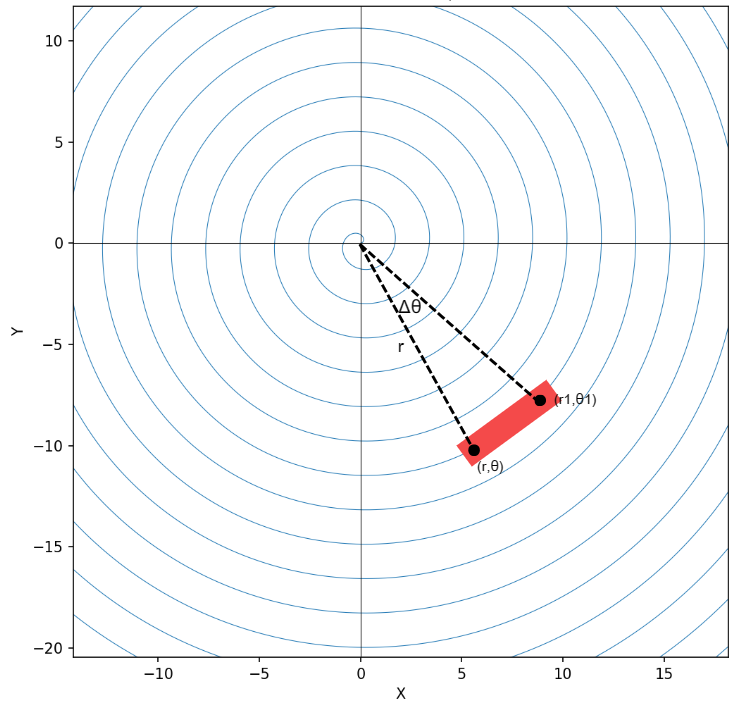
\includegraphics[width=\textwidth]{pics/dts}
		\subcaption{位置递推示意图(以第一节龙身为例)}
		\label{fig:dtd}
	\end{subfigure}
	\hfill
	\begin{subfigure}[t]{0.45\textwidth}
		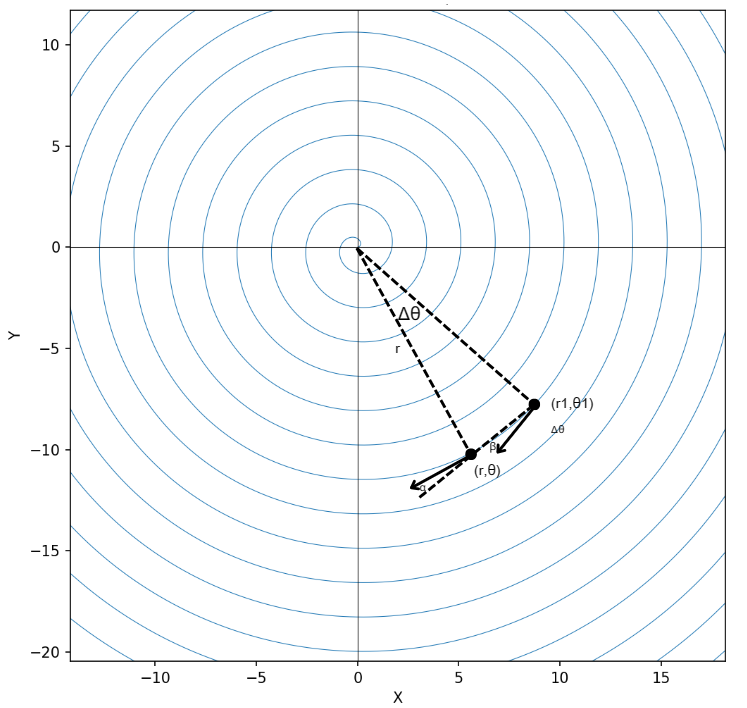
\includegraphics[width=\textwidth]{pics/dtv}
		\subcaption{速度递推示意图(以第一节龙身为例}
		\label{fig:dtv}
	\end{subfigure}
\end{figure}
以龙头递推第一节龙身前把手位置为例,第一节龙身前把手和原点连线与龙头把手和原点连线满足三角函数,其位置如图\ref{fig:dtd}所示
\begin{align*}
	L_0^2 = r_0^2 +r_1^2 - 2*r_0*r_1*cos(\triangle\theta)
\end{align*}
$v_1$为$s$关于$t$的导数的同时,也满足递推式
\begin{align*}
	v_0*sin(\pi-\alpha) = v_1*sin(\pi-\beta)
\end{align*}
递推可得
\begin{align*}
	v_1 &= v_0*\frac{sin\alpha}{sin\beta}=\frac{r_1}{r_0}\\
	v_2 &= v_1*\frac{sin\alpha}{sin\beta}= v_0*\frac{sin\alpha}{sin\beta}*\frac{r_2}{r_1}\\
v_i&= v_0*\frac{r_i}{r_0}
\end{align*}
在每秒通过龙头位置及其固定速度对各节点位置速度进行递推求解。

\subsection{问题一模型的求解}
将模型一的参数代入计算程序中进行求解,在通过$L_0^2 = r_0^2 +r_1^2 - 2*r_0*r_1*cos(\triangle\theta)$计算各把手行进位置过程中,采用基于Newton-Raphson的求数值解方法的$root$函数来确定未知$\triangle\theta$的值。考虑$cos\theta$具有$2\pi$为周期的周期性特征,设置函数在每次迭代时逼近$\theta_0-\triangle\theta$,即理论上的$\theta1$值,但由于所涉及到所有计算数值均较小,$\triangle\theta$由于数值方法与实际存在偏差,$cos\theta$在给定逼近值左右两边都有较接近值且在循环中难以每次都取到准确初值等多种原因,$root$函数计算结果出现部分点位置不精确的情况,如图\ref{fig:inacc}所示。
\begin{figure}[htbp!]
	\centering
	\begin{subfigure}[t]{0.45\textwidth}
		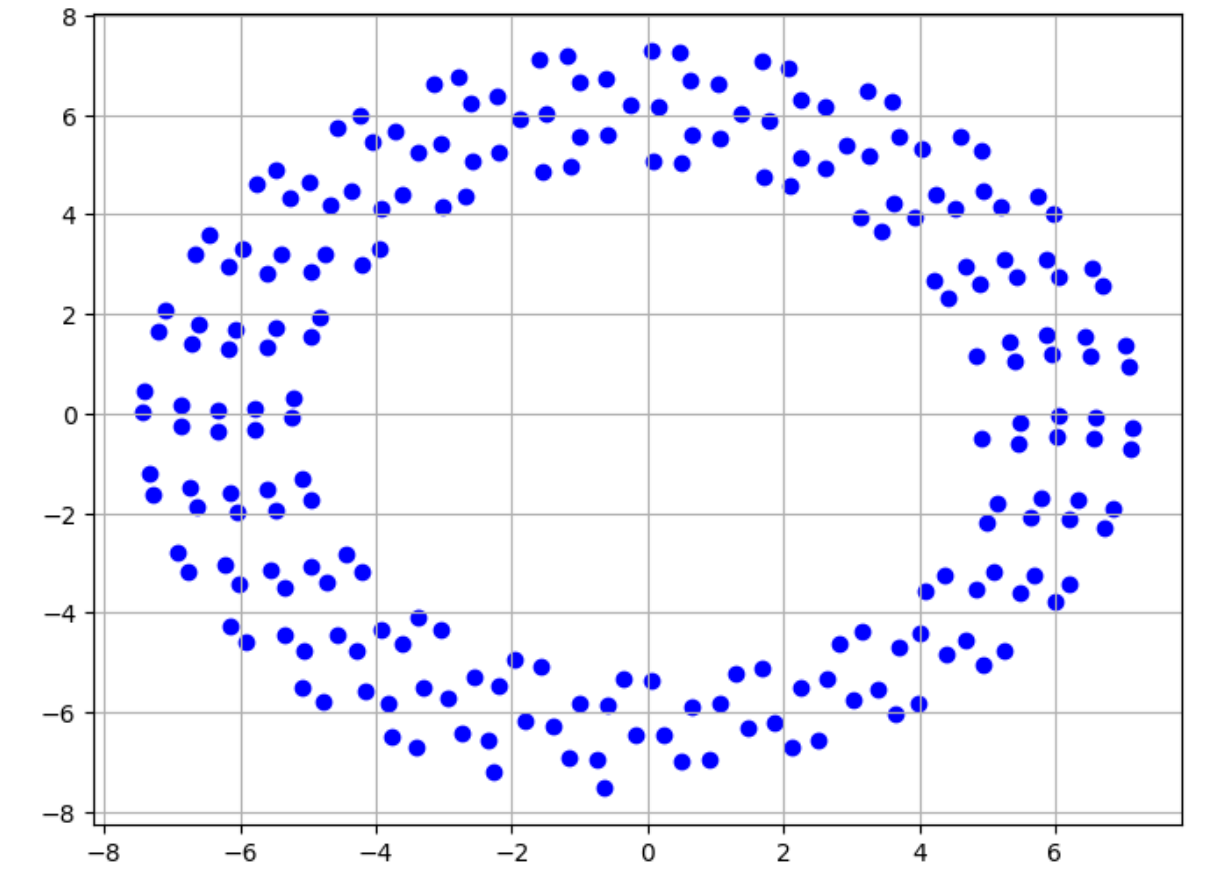
\includegraphics[width=\textwidth]{pics/inacc}
		\subcaption{牛顿迭代}
		\label{fig:inacc}
	\end{subfigure}
	\hfill
	\begin{subfigure}[t]{0.45\textwidth}
		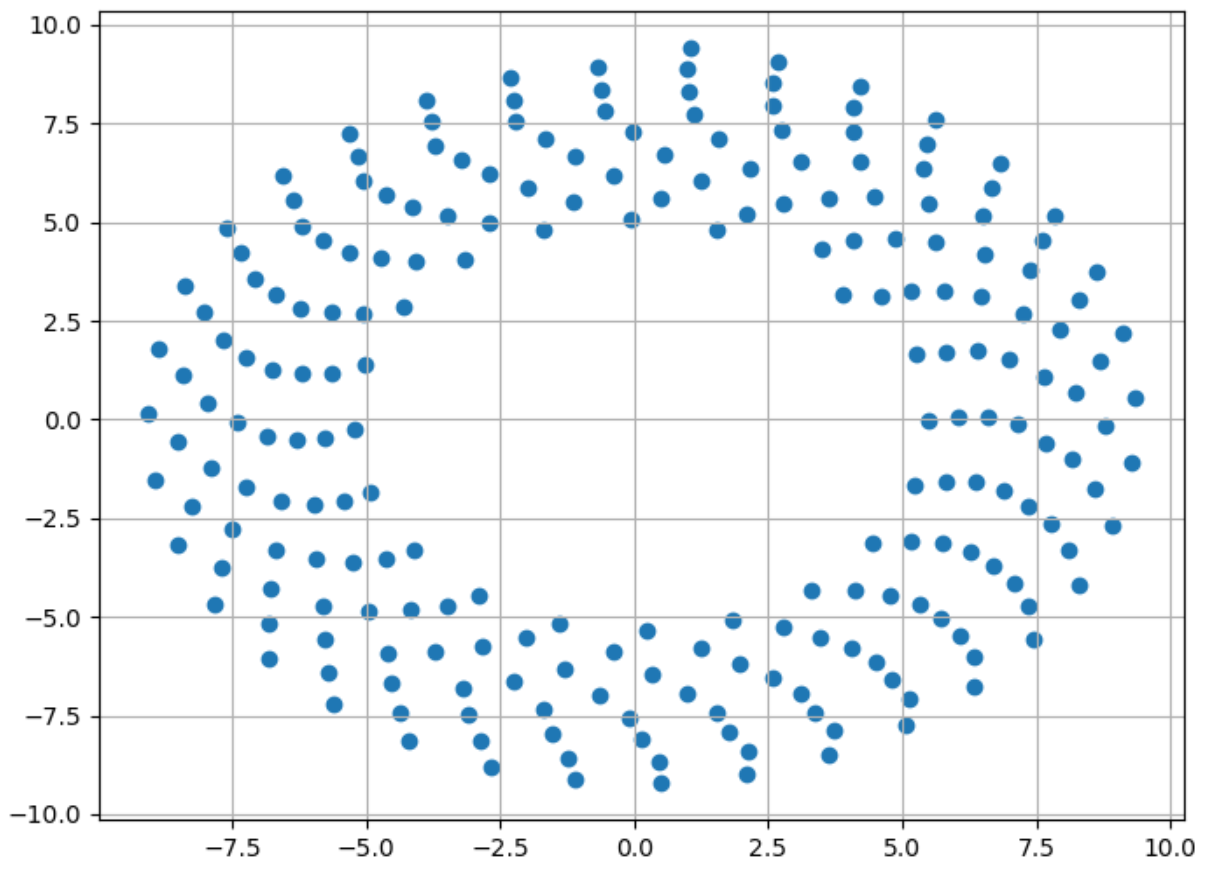
\includegraphics[width=\textwidth]{pics/acc}
		\subcaption{微元思想}
		\label{fig:qcc}
	\end{subfigure}
	\caption{不同思路下第$300s$各把手位置求解}
\end{figure}

因此,引入微元法相关思想,逆向对每个节点对应$\theta$值进行求解,设定步长$h=0.001$,每循环令弧度$\theta_{i+1}=\theta_i+h$。与此同时,令同在螺线上的两点距离(由欧式距离计算得出)与板凳有效长的差值为$\triangle L$(板凳有效长$L_0=2.86m$,其余$L=1.65m$),判断$\triangle L$是否$<0.01m$。

由于数据精度高,对于部分较难取到合适值的节点,在$\triangle L_i<0$且$\triangle L_{i}>0$时,将$\triangle L_{i+1}$与$\triangle L_{i}$ 的平均值作为节点的$\theta$,并在此基础上进行位置和速度递推,结果如表\ref{result11}和\ref{result12}所示:  
\begin{figure}[htbp!]
\centering
\begin{tabular}{|c|c|c|c|c|c|c|}
	\hline
	  & 0$s$ & 60$s$ & 120$s$ & 180$s$ & 240$s$ & 300$s$ \\ \hline
	龙头$x(m)$ & 8.800000 & 5.799209 & -4.084887 & -2.963609 & 2.594494 & 4.420274 \\ \hline
	% 继续添加直到15行
	龙头$y(m)$& 0.000000&-5.771092& -6.304479 & 6.09478 & -5.356743 & 2.320429 \\ \hline
	第1节龙身$x(m)$ & 8.363824 &7.456758& -1.445473 & -5.237118 & 4.821221 & 2.459489 \\ \hline
	第1节龙身$y(m)$ & 2.826544 & -3.440399 & -7.405883 & 4.359627 & -3.561949 & 4.402476 \\ \hline
	第51节龙身$x(m)$ & -9.515993 &-8.692692 & -5.536588 & 2.882407 & 5.998319 & -6.301432 \\ \hline
	第51节龙身$y(m)$ & 1.359255 & 2.518974 & 6.383524& 7.252598 & -3.799774 & 0.464845 \\ \hline
	第101节龙身$x(m)$ & 2.897887 & 5.703594 & 5.351534 & 1.919509 & -4.895743 & -6.241319 \\ \hline
	第101节龙身$y(m)$ & -9.922878 & -7.989866 & -7.564863 & -8.467164 & -6.396863& 3.93045 \\ \hline
	第151节龙身$x(m)$ & 9.305829 & 6.667084 & 2.406079 & 0.991941 & 2.941486 & 7.043423 \\ \hline
	第151节龙身$y(m)$ & 1.810861 & 8.147242 & 9.72298 & 9.426274 & 8.408382 & 4.388608 \\ \hline
	第201节龙身$x(m)$ & 4.578571 & -6.625884 & -10.62677 & -9.278034 & -7.442329 & -7.45391 \\ \hline
	第201节龙身$y(m)$ & 10.714911 & 9.021079 & 1.363073 & -4.268278 & -6.198897 & -5.270251 \\ \hline
	龙尾后$x(m)$ & -5.323877 & 7.368686 & 10.974251 & 7.366113 & 3.213866 & 1.783554 \\ \hline
	龙尾后$y(m)$ & -10.667235 & -8.794587 & 0.844882 & 7.510148 & 9.478864 & 9.301462 \\ \hline
\end{tabular}                                              
\caption{$result1$各节把手位置} 
\label{result11}                               
\end{figure}
\begin{figure}
	\centering
	\begin{tabular}{|c|c|c|c|c|c|c|}
		\hline
		& 0$s$ & 60$s$ & 120$s$ & 180$s$ & 240$s$ & 300$s$ \\ \hline
		龙头$(m/s)$ & 1.000000 & 1.000000 & 1.000000 & 1.000000 & 1.000000 & 1.000000 \\ \hline
		第1节龙身$(m/s)$ & 1.003242 & 1.003752& 1.004453 & 1.005476 & 1.00711 & 1.010133 \\ \hline
		第51节龙身$(m/s)$ & 1.092339 & 1.106197 & 1.124846 & 1.151579 & 1.192976 & 1.265656 \\ \hline
		第101节龙身$(m/s)$ & 1.174701 & 1.199879 & 1.233517 & 1.281078 & 1.353384 &1.477432 \\ \hline
		第151节龙身$(m/s)$ & 1.251643 & 1.286746 & 1.333338 & 1.398577 & 1.496651 & 1.66231 \\ \hline
		第201节龙身$(m/s)$ & 1.324108 & 1.368087 & 1.426196 & 1.506945 & 1.627322 & 1.828585 \\ \hline
		龙尾后$(m/s)$ & 1.35477 & 1.402383 & 1.465185 & 1.552223 & 1.681605 & 1.897099 \\ \hline
	\end{tabular}
	\caption{$result1$各节把手速度}   
	\label{result12}         
\end{figure}
\subsubsection{数据结果分析}
\begin{itemize}
	\item 对于同一节点不同时间
	\begin{itemize} 
		\item 同一节点轨迹为等距螺线。
		\item 除龙头前把手行进速度保持恒定外,其余把手节点速度随时间增大逐渐增长,且在相同时间差$\triangle t $内,越靠近龙尾的节点,速度增长越快,即加速度越大。
	\end{itemize}
	\item 对于同一时间不同节点
	\begin{itemize} 
		\item 整体轨迹呈等距螺线。
		\item 观察同一时刻所有节点,越靠近龙尾后把手节点速度越快,即从龙头至龙尾节点速度呈上升趋势。
	\end{itemize}
\end{itemize}

\subsection{问题二模型的建立}

在模拟板凳龙的运行过程中,可能发生碰撞的情况主要包括以下三种情形\cite{ref2}:
\begin{figure}[htbp!]
	\centering
	\begin{subfigure}[t]{0.32\textwidth}
		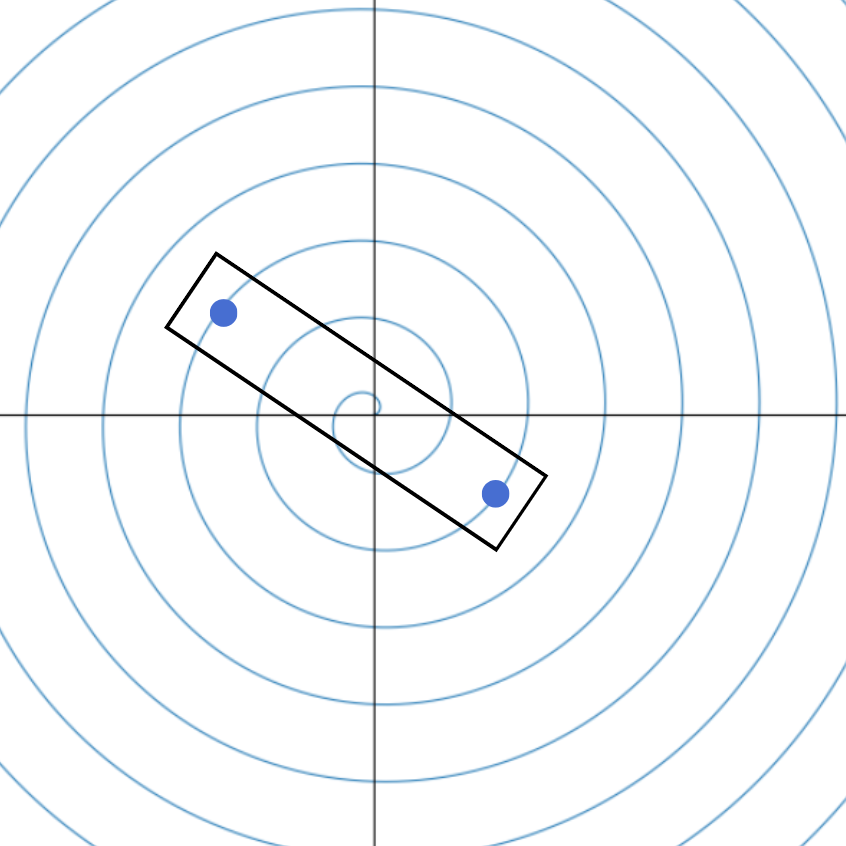
\includegraphics[width=\textwidth]{pics/s22}
		\subcaption{情况一示意图}
		\label{fig:cra1}
	\end{subfigure}
	\hfill
	\begin{subfigure}[t]{0.32\textwidth}
		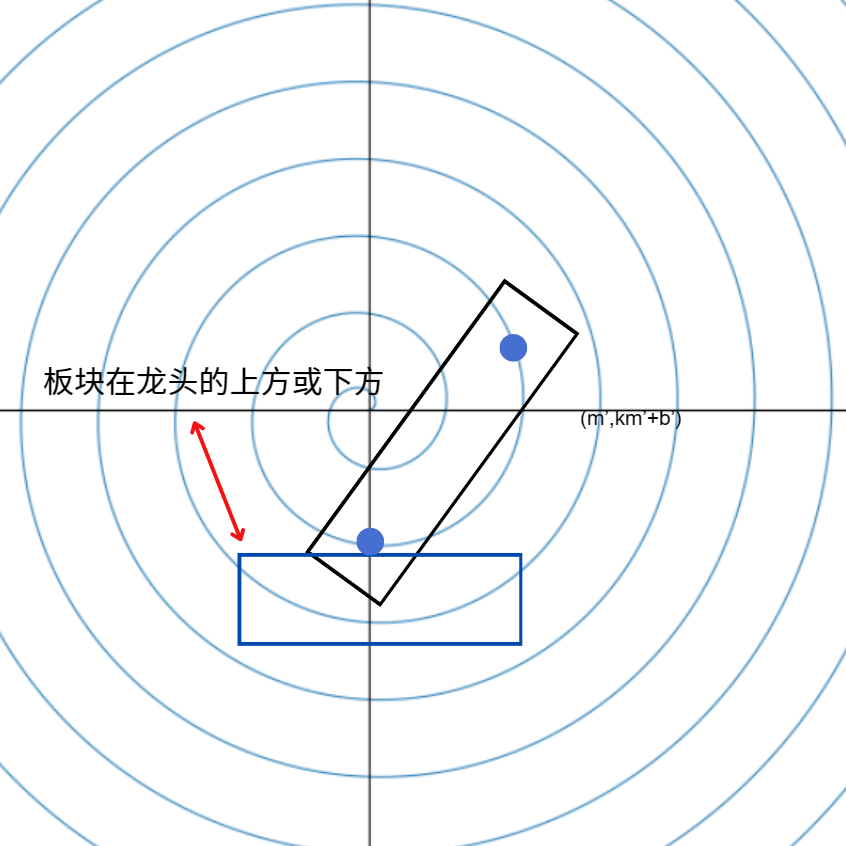
\includegraphics[width=\textwidth]{pics/s23}
		\subcaption{情况二示意图}
		\label{fig:cra2}
	\end{subfigure}\\
	\begin{subfigure}[t]{0.32\textwidth}
		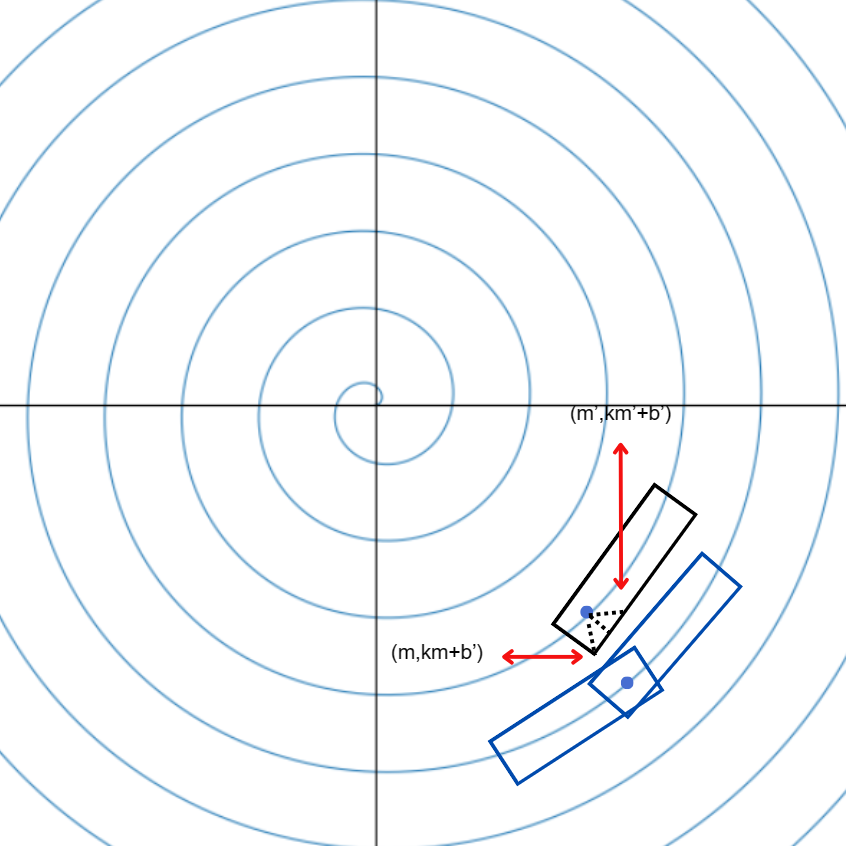
\includegraphics[width=\textwidth]{pics/s21}
		\subcaption{情况三示意图}
		\label{fig:cra3}
	\end{subfigure}
	\label{a}
\end{figure}
\begin{itemize}
	\item 直径卡滞模型:在板凳龙运行过程中,当龙头板凳近似成为螺线直径,龙头部位发生卡滞,无法再向前运行,如图\ref{fig:cra1}所示,此种情况满足: 
	\begin{align*}
		b\gamma + b(\gamma+\frac{\pi}{2}) = L_0
	\end{align*}
	\item 三维把碰板碰撞模型:在运行过程中假设由于相邻前后板凳拼接和手持把手舞龙人身高造成的的高度差,可能会出现龙头前把手与外圈板碰撞的情况,碰撞条件满足:
	\begin{align*}
		d_2 \leq w+\frac{D}{2}
	\end{align*}
	此处$d$指龙头把手中心相邻外圈的板凳的最近边的距离。
	\item 二维板碰板碰撞模型:在运行过程中假设不存在高度差,所有板凳运行在同一二维平面,可能会出现龙头板与外圈板碰撞的情况,碰撞条件满足以下方程,即
	\begin{align}
		d_3 \leq \frac{D}{2}
	\end{align}
	此处$d$指板头对应顶点A与相邻外圈的板凳的最近边的距离。
\end{itemize}

我们将分别计算三种潜在碰撞情况对应的时间,并从中确定最早发生碰撞的时间节点。

\subsection{问题二模型的求解}
\begin{itemize}
	\item 对于直径卡滞模型,可以由运算直接得出$\gamma$为2.7225,即$32\pi-2.7225$
	\item 对于三维把碰板碰撞模型:设龙头前把手坐标为$(x_0,y_0)$
	\begin{align*}
	d_2 =\frac{|Ax_0+By_0+C|}{\sqrt{A^2+B^2}} =0.1525
	\end{align*}
	\item 对于二维板碰板碰撞模型,推导运算过程如下,对于与龙头对应板碰撞的板块,存在两条平行的直线(板的两条长),设两条线段所在直线方程为
\begin{align*}
	kx - y + b &= 0 \\
	kx - y + b' &= 0 \\
	\frac{\lvert b' - b \rvert}{\sqrt{1 + k^2}} = d_2 &= 0.15 \, \text{m}
\end{align*}
	计算原点至两条直线分别的距离,始终保留离原点更远的直线,令选取直线为$kx - y + b' = 0$,在$	d_3 \leq \frac{D}{2}$条件下,求解横坐标$m$。
\begin{align*}
	\frac{D}{2}&= (m-x_0)^2 + (km+b'-y_0)^2 \\
	\frac{157}{1600}&=m^2-2mx_0+x_0^2+k^2m^2+2k(b'-y_0)*m++(b'-y_0)^2\\
	0&=(1+k^2)m^2+(2k(b'-y_0))m+x_0^2+(b'-y_0)^2-\frac{157}{1600}\\
	 \triangle&= (2k(b'-y_0)-2x_0)^2-4(1+k^2)*(x_0^2+(b'-y_0)^2)-\frac{157}{1600}
\end{align*}
可解得横坐标\\$$m_1 = \frac{2x_0-2k(b'-y_0)+\sqrt{\triangle}}{2(1+k^2)}, m_2 = \frac{2x_0-2k(b'-y_0)-\sqrt{\triangle}}{2(1+k^2)}$$

根据图\ref{fig:cra3}所示,非顶点在模拟过程中不会与其他物体发生碰撞。因此,我们将采用所有计算得到的$m$值,并将其应用于后续每个时间点的模拟计算中,以确定碰撞发生的具体位置和对应的时间点。经过计算得到龙头前把手、龙身第 1、51、101、151、201条龙身前把手和龙尾后把手的位置和速度如表\ref{fig:end}所示。
\begin{figure}
	\centering
	\begin{tabular}{|c|c|c|c|}
		\hline
		& \textbf{横坐标$x(m)$} & \textbf{纵坐标$y(m)$} & \textbf{速度$(m/s$} \\ \hline
		龙头$(m/s)$ & 3.299984 & 0.175616 & 1.000000 \\ \hline
		第1节龙身$(m/s)$ & 2.003351 & 2.7248 & 1.023407 \\ \hline
		第51节龙身$(m/s)$ & -0.490812 & 5.072253 & 1.542051 \\ \hline
		第101节龙身$(m/s)$ & -5.798 & -2.619167 & 1.925206 \\ \hline
		第151节龙身$(m/s)$ & -7.32615 & 1.122784 & 2.242803 \\ \hline
		第201节龙身$(m/s)$ & 5.026079 & 6.643861 & 2.520932 \\ \hline
		龙尾后$(m/s)$ & 4.102846 & -7.677999 & 2.634303 \\ \hline
	\end{tabular}
	\caption{终止时刻位置与速度} 
	\label{fig:end}          
\end{figure}
\end{itemize}




\subsection{问题三模型的建立与求解}
依据题目条件,建立同时满足瞬间把手中心$r = 4.5m$,螺距最小以及模型不碰撞的优化模型
\[
\left\{
\begin{aligned}
	\text{minimize}\quad p &= \frac{9\pi}{32\pi - \gamma_0}\\
	d &\geq 15+ \frac{5.5}{2}\\
	r &= 4.5
\end{aligned}
\right.
\]

通过综合分析第二问中得出的各类数据,并对其进行详尽的遍历处理,我们可以得到螺距所对应碰撞时间以及碰撞点所对应半径$r$如下:
\begin{figure}
	\centering
\begin{tabular}{|c|c|c|}
	\hline
	\textbf{螺距$(cm)$} & \textbf{半径$(m)$} & \textbf{碰撞时间$(s)$} \\ \hline
	50 & 1.878907823 & 380 \\ \hline
	51 & 2.10215711 & 383 \\ \hline
	52 & 2.415837767 & 383 \\ \hline
	53 & 2.508608406 & 389 \\ \hline
	54 & 3.056155576 & 380 \\ \hline
	55 & 3.304653981 & 380\\ \hline
	56 & 3.440907408 & 384 \\ \hline
	57 & 3.524476715 & 390 \\ \hline
	58 & 3.879076511 & 385 \\ \hline
	59 & 4.05479401 & 387 \\ \hline
	60 & 3.671860473 & 412 \\ \hline
	61 & 4.263836273 & 397 \\ \hline
	62 & 4.736351777 & 385 \\ \hline
\end{tabular}
	\caption{螺距大小与碰撞关系呈现}           
\end{figure}
由于题中给定调头空间是以螺线中心为圆心、直径为 9$m$的圆形区域,可得最小螺距约为$61.5cm$。
\subsection{问题四模型的建立}
由题意可得螺距$p$为 1.7 $m$,龙头前把手的行进速度始终保持1$m/s$盘出螺线与盘入螺线关于螺线中心呈中心对称,设定舞龙队在掉头空间内完成掉头。由基本不等式简单推理可得,当且两段圆弧经过同一条直线时,调头曲线变短,掉头路线如图\ref{fig:s1}所示。在前几问认知基础上,分三段建立模型对包括掉头过程在内的$-100-100s$位置和速度信息进行求解,三段分别如图\ref{fig:s1},\ref{fig:s2}和\ref{fig:s3}所示。
\begin{itemize}
	\item -100-0$s$:板凳龙整体沿螺线正常盘入,除龙头前把手外其他节点经历加速过程。
	\item 0$s$-龙头前把手出掉头区域时刻:龙头及前几节龙身进入掉头区域内。
	\item 龙头前把手出掉头区域时刻-100$s$:龙头部分前把手已超出了指定掉头区域,其余龙身部分继续沿同一路径前进。
\end{itemize}
\begin{figure}[htbp!]
	\centering
	\begin{subfigure}[t]{0.32\textwidth}
		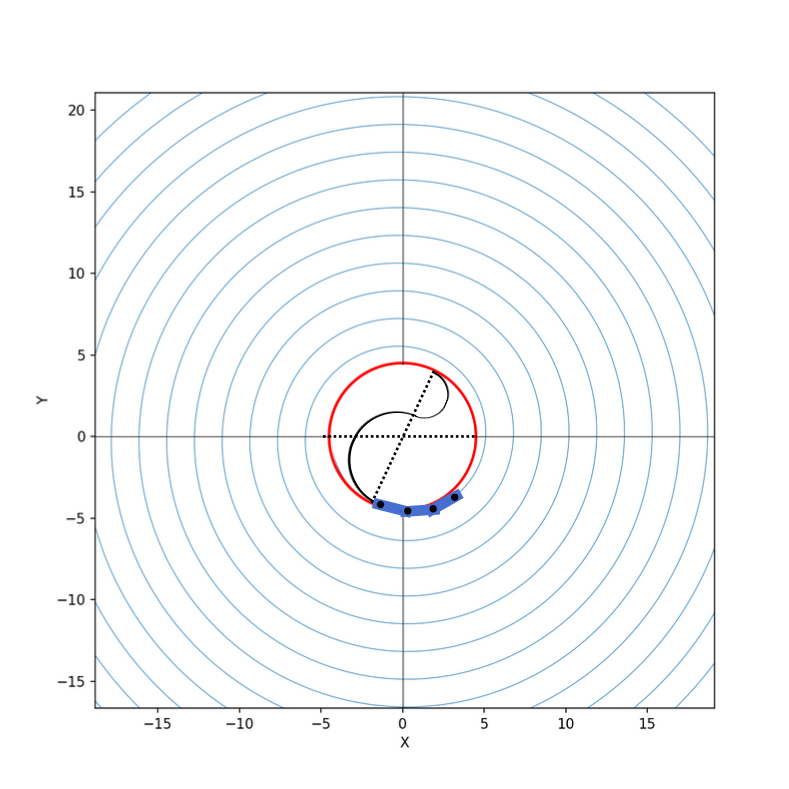
\includegraphics[width=\textwidth]{pics/sch1}
		\subcaption{情况一示意图}
		\label{fig:s1}
	\end{subfigure}
	\hfill
	\begin{subfigure}[t]{0.32\textwidth}
		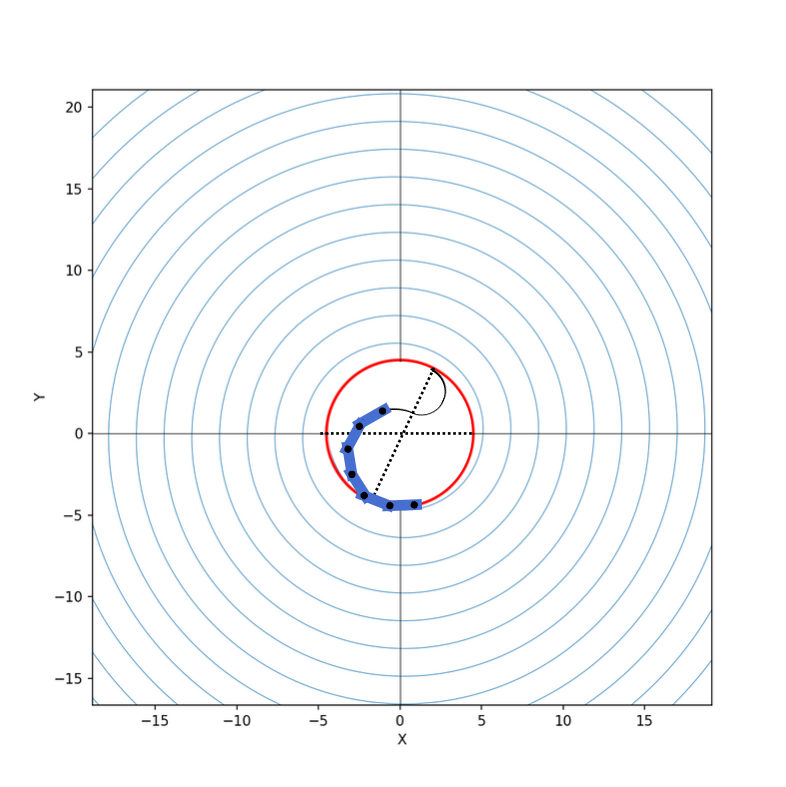
\includegraphics[width=\textwidth]{pics/sch2}
		\subcaption{情况二示意图}
		\label{fig:s2}
	\end{subfigure}
	\begin{subfigure}[t]{0.32\textwidth}
		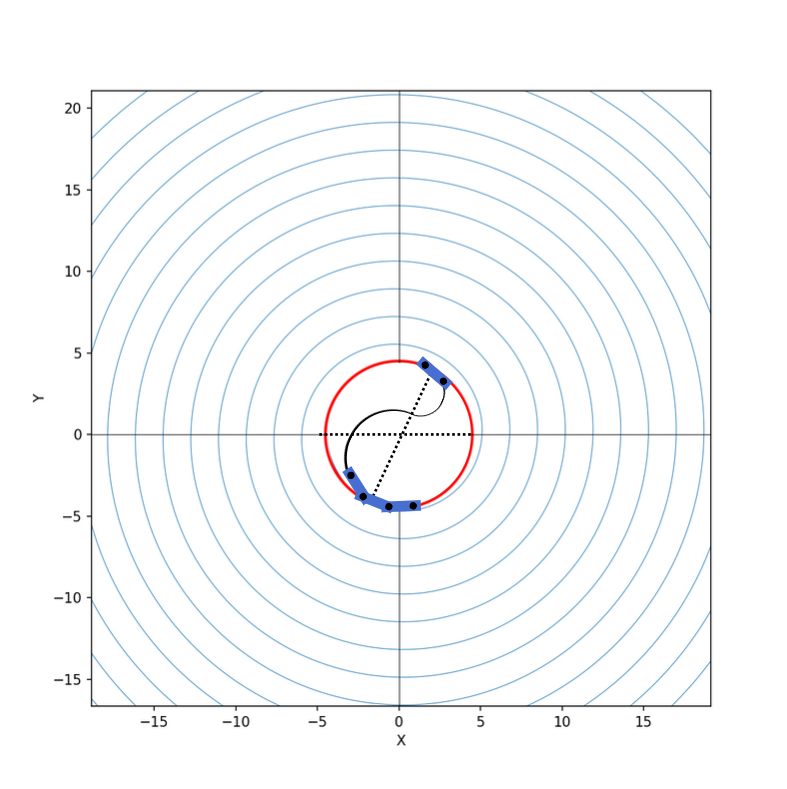
\includegraphics[width=\textwidth]{pics/sch3}
		\subcaption{情况三示意图}
		\label{fig:s3}
	\end{subfigure}
	\label{a}
\end{figure}
\subsubsection{阶段一模型的建立}
阶段一模型与问题一呈相同趋势,由图观察此时$a=0$,由螺距基本参数方程$r = b\gamma$,可得龙头前把手进去掉头区域时刻满足条件$\gamma = \frac{9\pi}{1.7}$。此时节点仍满足第一问递推关系:
\begin{align*}
	L_0^2 &= r_0^2 +r_1^2 - 2*r_0*r_1*cos(\triangle\theta)\\
	&v_0*sin(\pi-\alpha) = v_1*sin(\pi-\beta)
\end{align*}

据此可递推出$−100-0s$时任一节点的位置和速度。

\subsubsection{阶段二模型的建立}
根据最短掉头路径示意图求出掉头路线所需经历弧长为$\pi*(3+1.5) = 4.5\pi \approx 14.14m$,龙头前把手在掉头区域中的各时刻速度递推如下图\ref{tab:n1}所示

由于两段圆弧相切,由三角函数可推得步长:$$t' = \frac{2\pi arcsin(\frac{L}{2r})}{180\textdegree}*r \approx 1.6$$

通过进入掉头区域的最后一节龙身,可由盘入螺线递推出每点的位置和速度。
\begin{table}[h]
	\centering
	\begin{tabular}{|c|c|c|c|c|c|c|c|c|c|}
		\hline
		 & 0*$t'$ & 1*$t'$ & 2*$t'$ & 3*$t'$ & 4*$t'$ & 5*$t'$ & 6*$t'$ & 7*$t'$ & 8*$t'$ \\ \hline
	    龙头 & $v_0$ & $v_0$  &$v_0$ & $v_0$ & $v_0$ & $v_0$ & $v_0$ & $v_0$ & $v_0$ \\ \hline
		第一节龙身& $\frac{r_1}{r_0}*v_0$ & $v_0$ & $v_0$ & $v_0$ & $v_0$ & $v_0$ & $v_0$ & $v_0$ & $v_0$ \\ \hline
		第二节龙身 & $\frac{r_2}{r_0}*v_0$ & $\frac{r_1}{r_0}*v_0$ & $v_0$ & $v_0$ & $v_0$ & $v_0$ &$v_0$ & $v_0$ & $v_0$ \\ \hline
		第三节龙身 & $\frac{r_3}{r_0}*v_0$ & $\frac{r_2}{r_0}*v_0$ & $\frac{r_1}{r_0}*v_0$ & $v_0$ & $v_0$ & $v_0$ & $v_0$ & $v_0$ & $v_0$ \\ \hline
		第四节龙身 & $\frac{r_4}{r_0}*v_0$ & $\frac{r_3}{r_0}*v_0$3 & $\frac{r_2}{r_0}*v_0$ & $\frac{r_1}{r_0}*v_0$ & $v_0$ & $v_0$& $v_0$ & $v_0$ & $v_0$ \\ \hline
		第五节龙身 & $\frac{r_5}{r_0}*v_0$ & $\frac{r_4}{r_0}*v_0$ & $\frac{r_3}{r_0}*v_0$ & $\frac{r_2}{r_0}*v_0$ & $\frac{r_1}{r_0}*v_0$ & $v_0$ & $v_0$ & $v_0$ & $v_0$ \\ \hline
		第六节龙身 & $\frac{r_6}{r_0}*v_0$ & $\frac{r_5}{r_0}*v_0$ & $\frac{r_4}{r_0}*v_0$ & $\frac{r_3}{r_0}*v_0$ & $\frac{r_2}{r_0}*v_0$ & $\frac{r_1}{r_0}*v_0$ & $v_0$ & $v_0$ & $v_0$ \\ \hline
		第七节龙身 & $\frac{r_7}{r_0}*v_0$ & $\frac{r_6}{r_0}*v_0$ & $\frac{r_5}{r_0}*v_0$ & $\frac{r_4}{r_0}*v_0$ & $\frac{r_3}{r_0}*v_0$ & $\frac{r_2}{r_0}*v_0$ & $\frac{r_1}{r_0}*v_0$ & $v_0$ & $v_0$ \\ \hline
		第八节龙身 & $\frac{r_8}{r_0}*v_0$ & $\frac{r_7}{r_0}*v_0$ & $\frac{r_6}{r_0}*v_0$ & $\frac{r_5}{r_0}*v_0$ & $\frac{r_4}{r_0}*v_0$ & $\frac{r_3}{r_0}*v_0$ & $\frac{r_2}{r_0}*v_0$ & $\frac{r_1}{r_0}*v_0$ & $v_0$ \\ \hline
		第九节龙身 & $\frac{r_9}{r_0}*v_0$ & $\frac{r_8}{r_0}*v_0$ & $\frac{r_7}{r_0}*v_0$& $\frac{r_6}{r_0}*v_0$& $\frac{r_5}{r_0}*v_0$ & $\frac{r_4}{r_0}*v_0$ & $\frac{r_3}{r_0}*v_0$ &$\frac{r_2}{r_0}*v_0$  & $\frac{r_1}{r_0}*v_0$ \\ \hline
	\end{tabular}
	\caption{情况2各节点速度递推}
	\label{tab:n1}
\end{table}
\subsubsection{阶段三模型的建立}
当龙头前把手离开掉头区域瞬间,模型进入阶段2,该阶段时间$t$范围为$4.5\pi-110s$, 板凳龙整体始终有一部分处在盘出螺线,一部分处于掉头区域内,此时假设第$i-1$块板正在离开掉头区域,此时可由盘出螺线方程以及龙头前把手坐标递推出第$i-1$板前把手位置坐标$(r_i,\theta_i)$,根据盘入和盘出螺线的中心对称性可得$(r_i,\theta_i) = (r_{i+10},\theta_{i+10})$,继续进行递推可得任一把手位置。

针对速度$v$,可由盘出螺线方程同样通过问题1中递推公式从$v_0$逆推至$v_{i}$,同时根据圆弧上各点运动速度大小相等,可以得到$$v_{i} = v_{i+1} = v_{i+2} = ... =v_{i+9}$$

从$v_{i+9}$可由第一问得出的盘入螺线位置与速度递推公式,递推出任一节点的位置和速度。
\subsubsection{基于弧线半径调整的模型的建立}
由于在不同半径圆弧上减速运动的复杂性,以及问题四给出的“能否调整圆弧,仍保持各部分相切,使得调头曲线变短”的条件,可由基本不等式得出最短掉头轨迹为两个相切的半径$r = \frac{9}{4}m$的半圆。由轨迹对称性可得给定时间节点位置和速度呈现在表格 \ref{fig:result41}和 \ref{fig:result42}中。
\subsection{问题四模型的求解}
\begin{figure}[htbp!]
	\centering
	\begin{tabular}{|c|c|c|c|c|c|}
		\hline
		& -100$s$ & -50$s$ & 0$s$ & 50$s$ & 100$s$  \\ \hline
		龙头$x(m)$ & 8.114087 & 6.770785 & -3.368062 & 2.58018 & 1.107567  \\ \hline
		% 继续添加直到15行
		龙头$y(m)$& 2.821146 &0.956084 & -2.896377 & 5.703593 & 7.960922 \\ \hline
		第1节龙身$x(m)$ & 7.01429 &6.389503 & -2.73958 & 1.182728 & -1.128568  \\ \hline
		第1节龙身$y(m)$ & 5.095932 & 2.618487 & -3.567203 & 6.212519 & 8.033879\\ \hline
		第51节龙身$x(m)$ & -6.989585 &-5.015423 & -3.930349 & -5.347988 & -1.94745  \\ \hline
		第51节龙身$y(m)$ & -8.871894 & 7.573062 & -4.780576 & 6.302041 & -10.394022  \\ \hline
		第101节龙身$x(m)$ & -11.984064 & 11.581299 & 0.029986 & 5.433503 & 12.753724 \\ \hline
		第101节龙身$y(m)$ & 10.532876 & -2.475983 & -8.075949 & -9.296725 & -6.516722\\ \hline
		第151节龙身$x(m)$ & -23.87089 & 4.846491 & 3.816306 & 9.226953 & -23.760469\\ \hline
		第151节龙身$y(m)$ & -6.427809 & -19.446249 & 9.808317 & 11.432272 & -1.668312  \\ \hline
		第201节龙身$x(m)$ & 6.351661 & 18.048186 & -9.830684 & -13.320931 & -19.82267 \\ \hline
		第201节龙身$y(m)$ & 26.820232 & -17.715751 & 10.290198 & -20.043436 & 18.329168 \\ \hline
		龙尾后$x(m)$ & 13.103671 & -13.656628 & 16.710078 & -24.43103 & 28.019657 \\ \hline
		龙尾后$y(m)$ & -25.425744 & -0.711752 & -11.416788 & -7.585207 & -1.061458\\ \hline
	\end{tabular}                                              
	\caption{$result4$各节把手位置} 
	\label{fig:result41}                               
\end{figure}
\begin{figure}
	\centering
	\begin{tabular}{|c|c|c|c|c|c|}
		\hline
		& -100$s$ & -50$s$ & 0$s$ & 50$s$ & 100$s$ \\ \hline
		龙头$(m/s)$ & 1.000000 & 1.000000 & 1.000000 & 1.000000 & 1.000000 \\ \hline
		第1节龙身$(m/s)$ & 0.9919 & 0.994181 & 0.996014 & 0.994725 & 0.992603  \\ \hline
		第51节龙身$(m/s)$ & 0.724356 & 0.805803 & 0.874862 & 0.834815 & 0.750042 \\ \hline
		第101节龙身$(m/s)$ & 0.249258 & 0.567113 & 0.739656 & 0.62866 & 0.374337 \\ \hline
		第151节龙身$(m/s)$ & -0.644395 & -0.141937 & 0.564228 & 0.305498 & -0.544494  \\ \hline
		第201节龙身$(m/s)$ & -0.934004 & -0.595917 & 0.298662 & -0.466748 & -0.847696  \\ \hline
		龙尾后$(m/s)$ & -1.040194 & 1.402383 & -0.13167 & -0.591555 & -0.949202  \\ \hline
	\end{tabular}
	\caption{$result4$各节把手速度}   
	\label{fig:result42}         
\end{figure}


%\subsection{龙格库塔法简介}
%龙格库塔法\cite{ref5}是一类解微分方程的数值算法, 其中较常见的是四阶龙格库塔法,其精度较高,这里不进行推导,仅仅给出公式:
%\begin{align*}
%	\begin{cases}
%		y_{k+1} = y_k + \dfrac{h}{6}(k_1+2k_2+2k_3+k_4) \\
%		k_{1} = f(t_k,y_k)\\
%		k_{2} = f(t_k+\frac{h}{2},y_k+\frac{h}{2}k_1)\\
%		k_{3} = f(t_k+\frac{h}{2},y_k+\frac{h}{2}k_2)\\
%		k_{4} = f(t_k+h,y_k+k_3)
%	\end{cases}
%\end{align*}
%之后我们将微分方程组带入MATLAB并利用四阶龙格库塔古典模型求解。
\newpage
\subsection{问题五模型的建立与求解}
基于问题四四个模型与掉头过程的分析,推断出当龙头前把手进入掉头过程的瞬间,龙尾后把手达到整个掉头过程中所有节点速度的最大值,因此再次运用在螺线$r=\frac{1.7}{2\pi}*\gamma$上速度的递推关系。当龙头进入掉头区域瞬间,龙尾后把手速度为$2m/s$时,龙头行进速度最大。
$$\frac{r_{223}}{r_{0max}}*v_0 = 2m/s$$$$v_0\approx 0.4447m/s$$

因此,使得舞龙队各把手的速度均不超过 $2m/s$的最大龙头速度约为$0.4447m/s$。
\section{模型的评价,改进与推广}
\subsection{模型的评价}
\subsubsection{优点}
\begin{itemize}
	\item 数据较为精确,运用牛顿迭代,微元法等多个方法进行比较分析,求解每秒整个舞龙队的位置和速度。
	\item 该模型设计考虑了广泛的适用性,从二维和三维两个不同维度考虑板凳的碰撞情况情况。
	\item 该模型具有较高的灵活性,能够根据不同的步长、螺距以及时间变量进行较为便捷的调整。
\end{itemize}
\subsubsection{缺点}
\begin{itemize}
	\item 将龙头划出掉头空间后后续节点在圆弧上的变速看为匀减速,数值会存在一定偏差。
	\item 模型四为简化模型,未考虑掉头路线的两个相切圆弧半径不同对于整个模型的影响。
	\item 本模型假设了相对严格的板间位置,未考虑板前后之间的拉扯产生的形变以及铆钉之间缝隙对板凳龙各节点速度的影响。
\end{itemize}
\subsection{模型的改进与推广}
\begin{itemize}
	\item 本题将模型进入盘入螺线前的轨迹均设定为相同螺距等螺距曲线的外圈,在生活中,可能存在各种进入队形的不规则路径。可从不同进入轨迹出发,讨论板凳龙演出的最优路径。
	\item 在本研究中,所采用的模型主要依赖于离散数值方法对变量进行逼近和求解。可考虑采用拟合方法,将离散数据点与适当的数学函数表达式相匹配,构建一个连续的函数模型,从而为变量间的关系提供更精确的描述。在有助于读者深入理解变量之间的动态关联的同时,使模型更具有普适性。
	\end{itemize}



\section{模型的检验}
基于本题建立的模型,我们可以从数值方法精度,边界条件和变化趋势上来证明其可行性和准确性。

%\subsection{敏感性分析}


\subsection{方法精度检验}
本文在推论过程中运用牛顿迭代的数值求解方法,由于文章内式子的解析解难以获得,以$\frac{\partial y}{\partial x} = \frac{2y}{t}+4t^2cos(4t)$这个易得出解析解的偏微分方程为例,求误差以及收敛阶如下图所示:
\begin{figure}[htbp!]
	\centering
		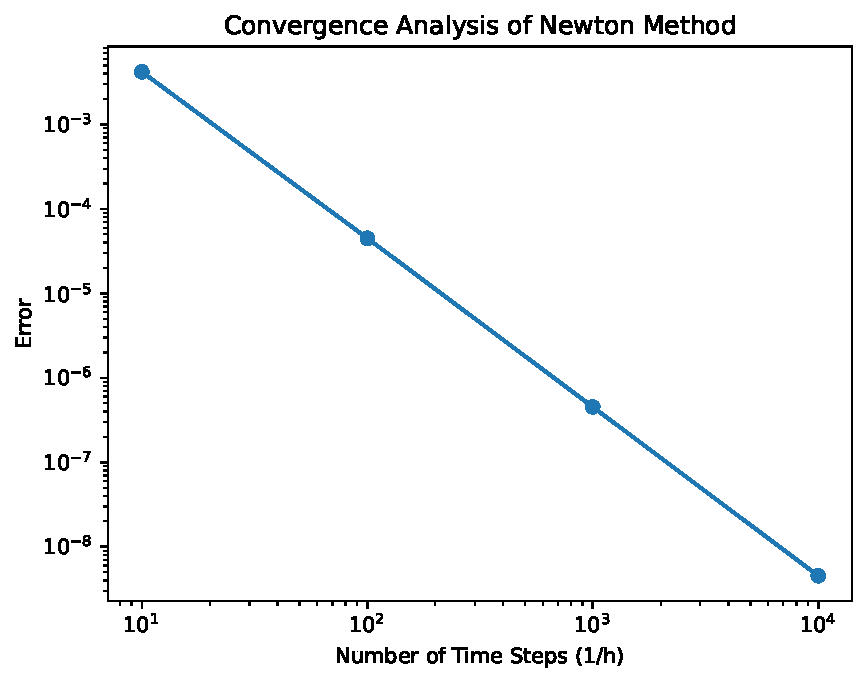
\includegraphics[width=0.5\textwidth]{pics/newton}
		\subcaption{牛顿迭代收敛}
		\label{fig:newton}
\end{figure}
\begin{figure}[htbp!]
	\centering
\begin{tabular}{|c|c|c|c|}
	\hline
Step Size & Error & Convergence Rate & Runtime \\ \hline
1.00e-01 & 4.20e-03  & 0.0000& 0.00 \\ \hline
1.00e-02 & 4.50e-05 & 1.9705 & 0.00 \\ \hline
1.00e-03 & 4.53e-07  & 1.9971 & 0.01 \\ \hline
1.00e-04  & 4.53e-09 & 1.9997 & 0.04 \\ \hline
\end{tabular}
\end{figure}

由此证明牛顿迭代具有二阶精度,计算坐标数值较为准确。
\subsection{边界条件检验}
验证模型在初始和最终时刻的状态是否符合预期,我们再次确认了代码算出的龙头的初始速度$v_0=0$和位置$(8.8, 0)$等端点数值,这些计算结果与模型的预期行为相吻合,从而验证了模型在边界条件下的有效性和准确性。
\subsection{变化趋势检验}
在第一二题目条件下,由于盘入运动的单项性,在分析把手的角位置(行进弧度)$\theta$,我们观察到每个把手的$\theta$始终小于其前一个把手值。因此对于任意给定的时刻,把手的$\theta$值呈现出递减趋势。这种排列方式与所提供的数据一致,验证了把手角位置的递减性假设。
\begin{figure}[htbp!]
	\centering
	\begin{subfigure}[t]{0.45\textwidth}
		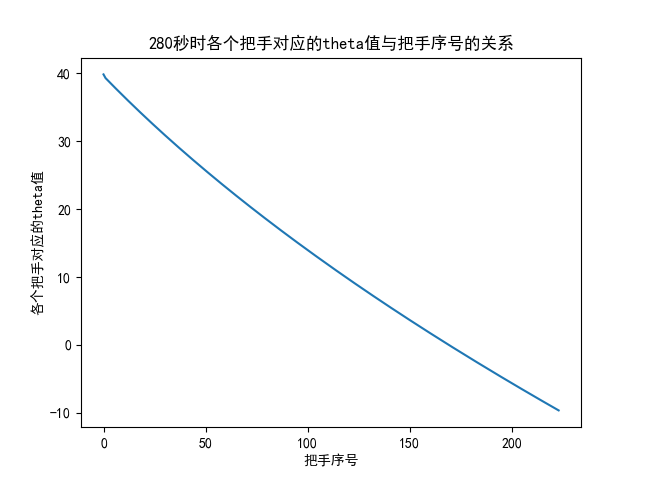
\includegraphics[width=\textwidth]{pics/a1}
		\subcaption{280$s$时各个把手对应的$\theta$值与把手序号的关系}
		\label{fig:a1}
	\end{subfigure}
	\hfill
	\begin{subfigure}[t]{0.45\textwidth}
		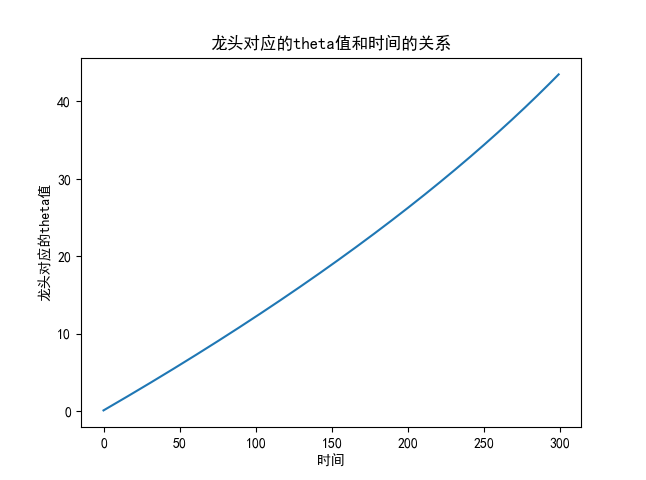
\includegraphics[width=\textwidth]{pics/b1}
		\subcaption{龙头对应的$\theta$值和时间的关系}
		\label{fig:b1}
	\end{subfigure}
\end{figure}





\newpage
\newpage
\begin{thebibliography}{99}  
	\bibitem{ref1}Banner, A. D. The calculus lifesaver : all the tools you need to excel at calculus. Princeton University Press, 2007.
	\bibitem{ref2}王栋, 周可璞. 基于阿基米德螺线走法的全区域覆盖路径规划 / Path Planning of the District Board Based on Archimedes’ Spiral. 工业控制计算机 / Industrial Control Computer, 2018, 31(5), 83–87.
	\bibitem{ref3}郑立飞, 魏宁, 万阿英. 如何用元素法解决阿基米德螺线的弧长. 呼伦贝尔学院学报 / JOURNAL OF HULUNBEIER UNIVERSITIES, 2021, 19(2):95-97.
%	\bibitem{ref4}尼古拉斯·迪方佐. 谣言心理学[A]. 机械工业出版社,2021:8.
%	\bibitem{ref5}房少梅,王霞. 微分方程数值解[A]. 国防工业出版社,2016:5.
\end{thebibliography}
%	\setcounter{page}{\value{savepage}} % 恢复保存的页码
\begin{appendices}
\pagestyle{plain} % 将页码样式设置为 plain

%\pagestyle{empty}
\section*{}
\newpage
\textbf{\textcolor[rgb]{0.00,0.00,0.00}{程序一:Python模拟问题一盘入曲线位置与速度}}
\lstinputlisting[language=Matlab]{./code/Question1.py}

\textbf{\textcolor[rgb]{0.00,0.00,0.00}{程序二:Python模拟问题二盘入终止时刻}}
\lstinputlisting[language=Matlab]{./code/Question2.py}

\textbf{\textcolor[rgb]{0.00,0.00,0.00}{程序三:Python模拟问题三最小螺距}}
\lstinputlisting[language=Matlab]{./code/Question3.py}

\textbf{\textcolor[rgb]{0.00,0.00,0.00}{程序四:Python模拟问题四掉头路径}}
\lstinputlisting[language=Matlab]{./code/Question4.py}
%
%\textbf{\textcolor[rgb]{0.00,0.00,0.00}{程序五:MATLAB模拟不同$\mu$对谣言传播的影响(模型1):}}
%\lstinputlisting[language=Matlab]{./code/SIR_RK4classic_a.m}
%
%\textbf{\textcolor[rgb]{0.00,0.00,0.00}{程序六:程序五对应微分方程组:}}
%\lstinputlisting[language=Matlab]{./code/ValueRu_a.m}
%
%\textbf{\textcolor[rgb]{0.00,0.00,0.00}{程序七:MATLAB模拟中途$\mu$有改变的情况(模型1):}}
%\lstinputlisting[language=Matlab]{./code/SIR_classic2mu.m}
%
%\textbf{\textcolor[rgb]{0.00,0.00,0.00}{程序八:程序七对应微分方程组1:}}
%\lstinputlisting[language=Matlab]{./code/ValueRu_1.m}
%
%\textbf{\textcolor[rgb]{0.00,0.00,0.00}{程序八:程序七对应微分方程组2:}}
%\lstinputlisting[language=Matlab]{./code/ValueRu_2.m}
%
%\textbf{\textcolor[rgb]{0.00,0.00,0.00}{程序九:MATLAB模拟谣言传播情况(模型2):}}
%\lstinputlisting[language=Matlab]{./code/SIRJW_RK4classic.m}
%
%\textbf{\textcolor[rgb]{0.00,0.00,0.00}{程序十:程序九对应微分方程组:}}
%\lstinputlisting[language=Matlab]{./code/ValueRu5.m}


%\newpage
%\def\thesection{A}
%\renewcommand{\thetable}{\wuhao A-\arabic{table}}
%\setcounter{table}{0}
%\section*{数据表格}
%\textcolor[rgb]{0.98,0.00,0.00}{\textbf{表格数据:}}
%\input{Appendices1}
%\begin{figure}[htbp!]
%	\centering
%	\begin{tabular}{|c|c|c|c|c|c|}
%		\hline
%		& -100$s$ & -50$s$ & 0$s$ & 50$s$ & 100$s$  \\ \hline
%		龙头$x(m)$ & 8.800000 & 5.799209 & -4.084887 & -2.963609 & 2.594494  \\ \hline
%		% 继续添加直到15行
%		龙头$y(m)$& 0.000000&-5.771092& -6.304479 & 6.09478 & -5.356743 \\ \hline
%		第1节龙身$x(m)$ & 8.363824 &7.456758& -1.445473 & -5.237118 & 4.821221  \\ \hline
%		第1节龙身$y(m)$ & 2.826544 & -3.440399 & -7.405883 & 4.359627 & -3.561949\\ \hline
%		第51节龙身$x(m)$ & -9.515993 &-8.692692 & -5.536588 & 2.882407 & 5.998319  \\ \hline
%		第51节龙身$y(m)$ & 1.359255 & 2.518974 & 6.383524& 7.252598 & -3.799774  \\ \hline
%		第101节龙身$x(m)$ & 2.897887 & 5.703594 & 5.351534 & 1.919509 & -4.895743 \\ \hline
%		第101节龙身$y(m)$ & -9.922878 & -7.989866 & -7.564863 & -8.467164 & -6.396863\\ \hline
%		第151节龙身$x(m)$ & 9.305829 & 6.667084 & 2.406079 & 0.991941 & 2.941486\\ \hline
%		第151节龙身$y(m)$ & 1.810861 & 8.147242 & 9.72298 & 9.426274 & 8.408382  \\ \hline
%		第201节龙身$x(m)$ & 4.578571 & -6.625884 & -10.62677 & -9.278034 & -7.442329  \\ \hline
%		第201节龙身$y(m)$ & 10.714911 & 9.021079 & 1.363073 & -4.268278 & -6.198897  \\ \hline
%		龙尾后$x(m)$ & -5.323877 & 7.368686 & 10.974251 & 7.366113 & 3.213866\\ \hline
%		龙尾后$y(m)$ & -10.667235 & -8.794587 & 0.844882 & 7.510148 & 9.478864\\ \hline
%	\end{tabular}                                              
%	\caption{$result4$各节把手位置} 
%	\label{result41}                               
%\end{figure}
%\begin{figure}
%	\centering
%	\begin{tabular}{|c|c|c|c|c|c|}
%		\hline
%		& -100$s$ & -50$s$ & 0$s$ & 50$s$ & 100$s$ \\ \hline
%		龙头$(m/s)$ & 1.000000 & 1.000000 & 1.000000 & 1.000000 & 1.000000 \\ \hline
%		第1节龙身$(m/s)$ & 1.003242 & 1.003752& 1.004453 & 1.005476 & 1.00711  \\ \hline
%		第51节龙身$(m/s)$ & 1.092339 & 1.106197 & 1.124846 & 1.151579 & 1.192976 \\ \hline
%		第101节龙身$(m/s)$ & 1.174701 & 1.199879 & 1.233517 & 1.281078 & 1.353384  \\ \hline
%		第151节龙身$(m/s)$ & 1.251643 & 1.286746 & 1.333338 & 1.398577 & 1.496651  \\ \hline
%		第201节龙身$(m/s)$ & 1.324108 & 1.368087 & 1.426196 & 1.506945 & 1.627322  \\ \hline
%		龙尾后$(m/s)$ & 1.35477 & 1.402383 & 1.465185 & 1.552223 & 1.681605  \\ \hline
%	\end{tabular}
%	\caption{$result4$各节把手速度}   
%	\label{result42}         
%\end{figure}
\end{appendices}
\end{document}